\documentclass[12pt]{article}
\setlength{\parindent}{0in}
\setlength{\parskip}{\baselineskip}

\usepackage[top=0.75in, bottom=0.75in, left=1in, right=1in]{geometry}

\usepackage{amsmath,amsfonts,amssymb,graphicx, hyperref, float}

\begin{document}

IBEHS 4A03 \hfill Assignment \#3\\
Baoze Lin, Hady Ibrahim

\hrulefill

% Custom numbering for subparts (e.g., 2.1, 2.2)
\renewcommand{\theenumii}{\arabic{enumi}.\arabic{enumii}}

\begin{enumerate}
  \item Question 1
    \begin{enumerate}
    
      % Answer to 1.1
      \item 
      The Routh array was constructed by first rewriting the characteristic equation of the closed-loop system using the substitution $T_I = \frac{1}{\tau_I}$ to simplify the algebra. The goal was to determine the range of $K_C$ and $\tau_I$ values that lead to a stable system based on Routh-Hurwitz criteria.
  
      \begin{figure}[H]
        \centering
        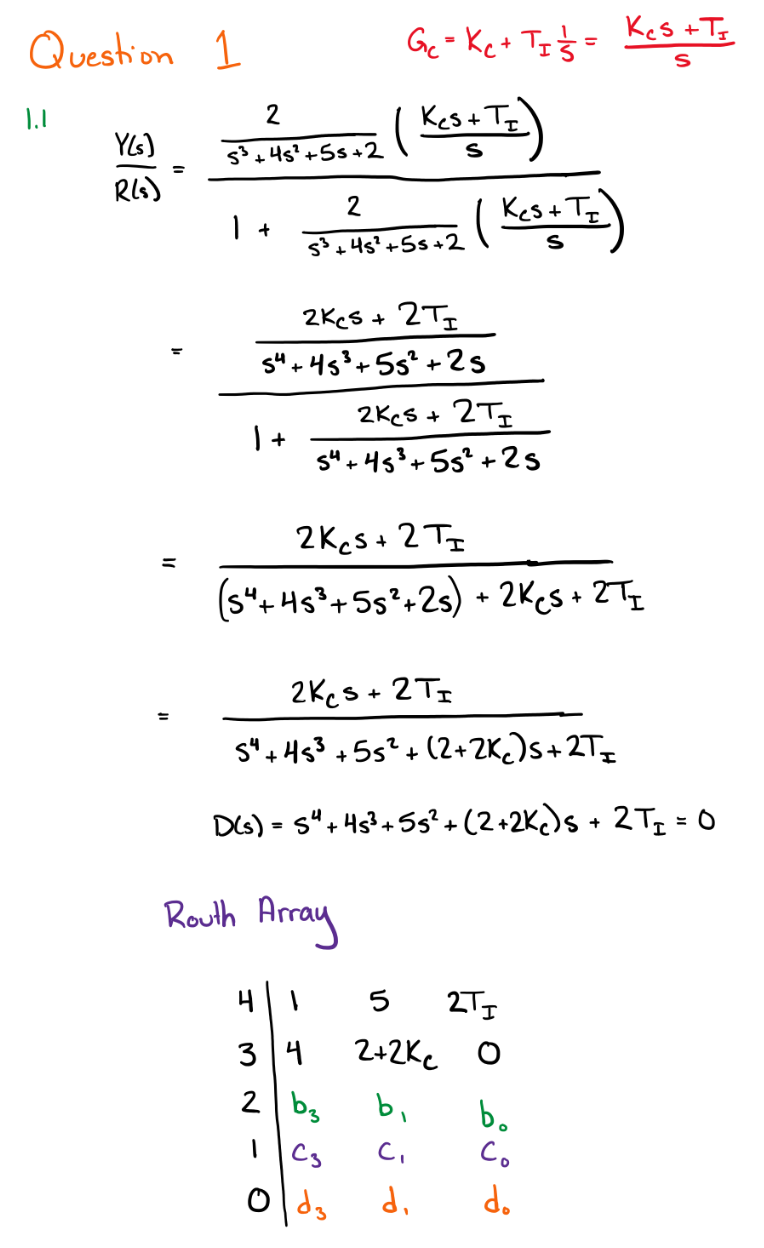
\includegraphics[width=0.6\textwidth]{Figures/figure1-1a.png}
        \caption{Step 1 of Routh Array derivation.}
      \end{figure}
  
      \begin{figure}[H]
        \centering
        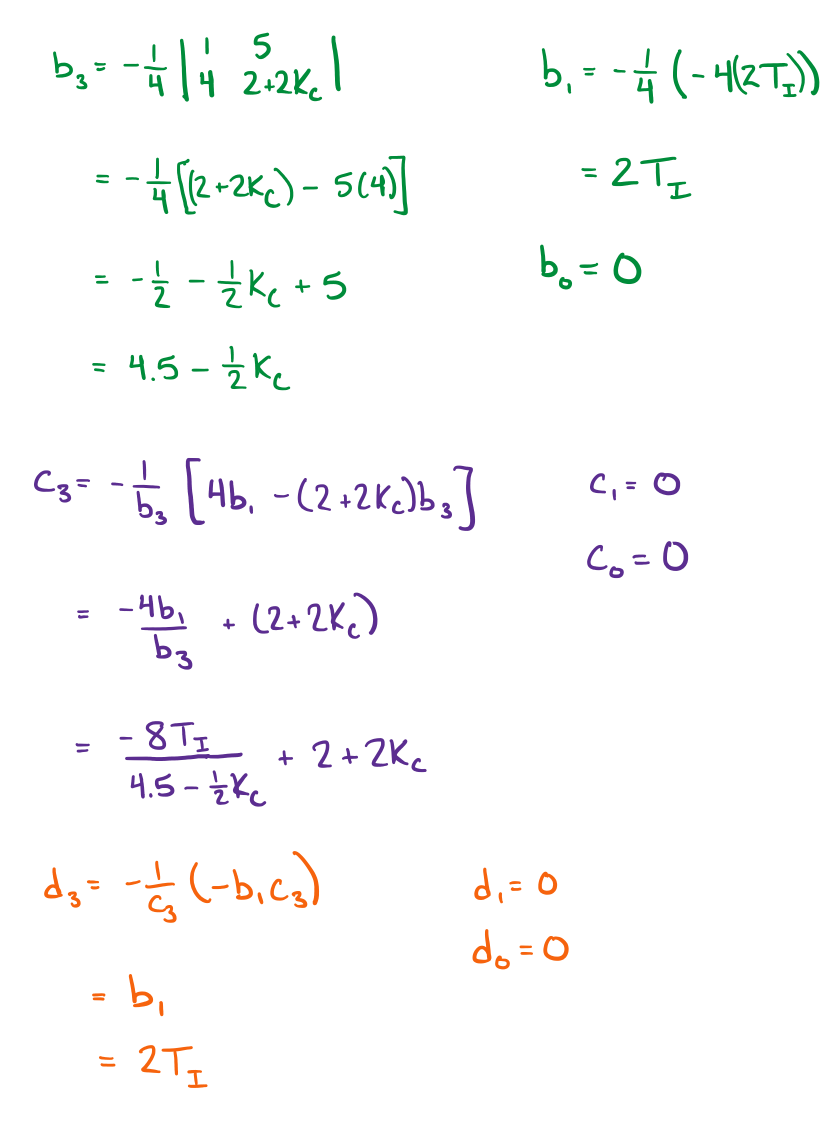
\includegraphics[width=0.7\textwidth]{Figures/figure1-1b.png}
        \caption{Step 2 of Routh Array derivation.}
      \end{figure}
  
      \begin{figure}[H]
        \centering
        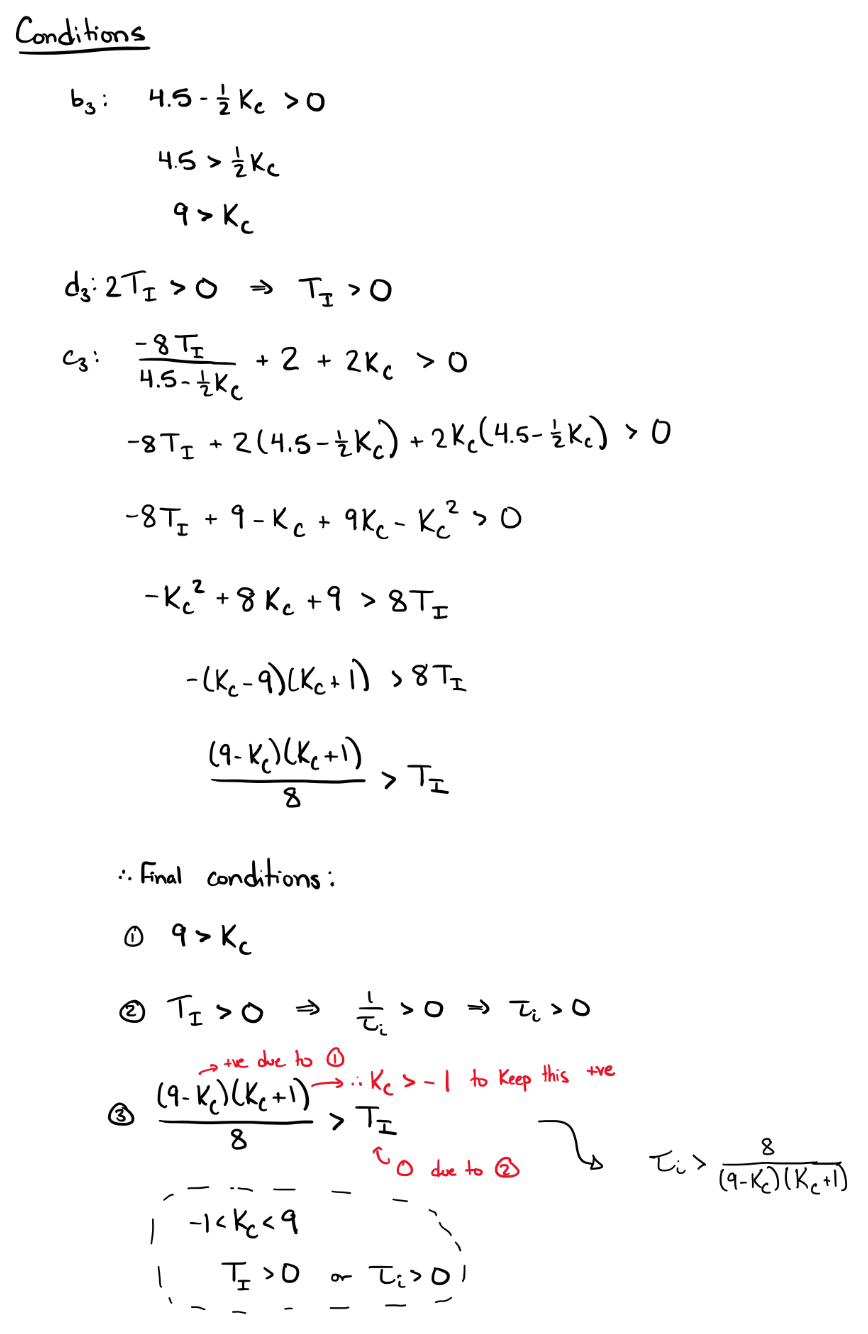
\includegraphics[width=0.7\textwidth]{Figures/figure1-1c.png}
        \caption{Final Routh Array with derived inequalities for stability.}
      \end{figure}
  
      \clearpage
      % Answer to 1.2
      \item 
      Using the inequalities derived in 1.1, the feasible set was plotted to visualize combinations of $K_C$ and $\tau_I$ that result in closed-loop stability. The red shaded region indicates infeasible (unstable) parameter combinations.
  
      \begin{figure}[H]
        \centering
        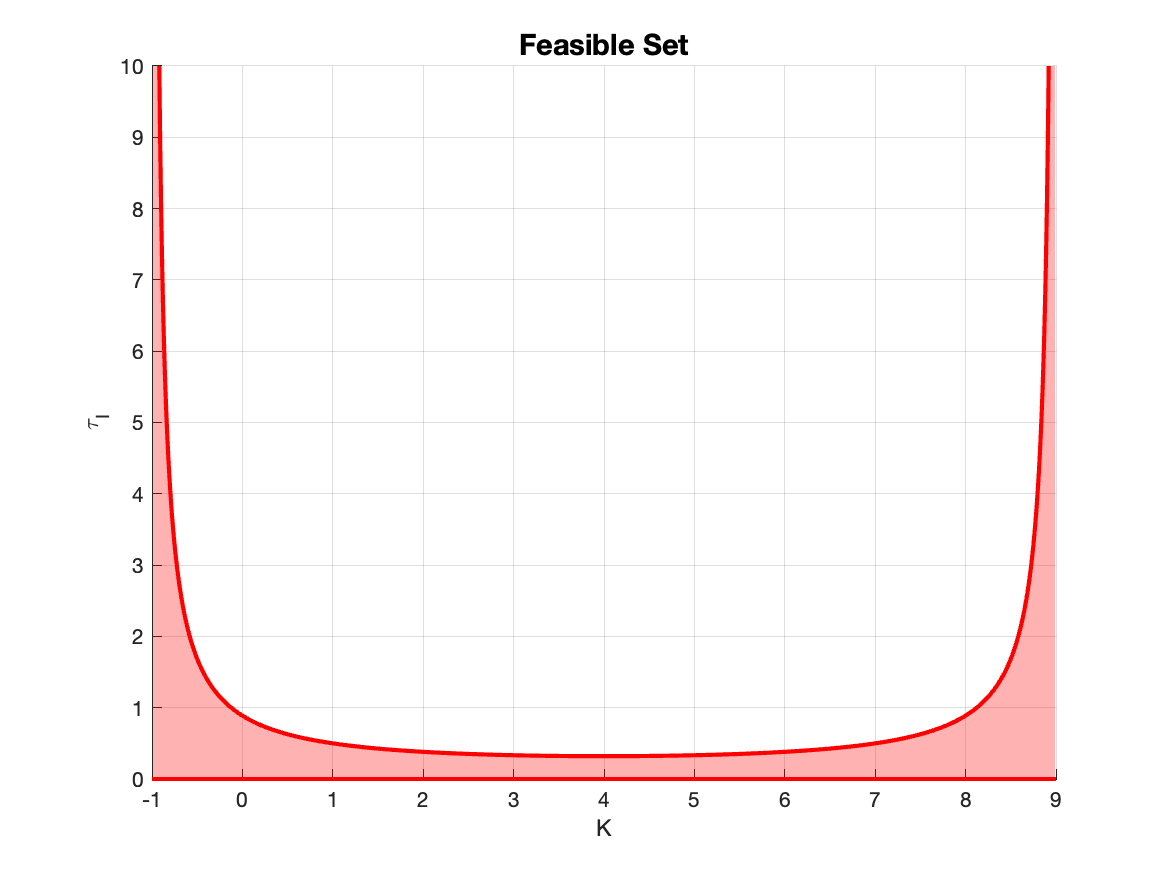
\includegraphics[width=0.8\textwidth]{Figures/figure1-2a.png}
        \caption{Feasible set for $K_C$ and $\tau_I$ from Routh-Hurwitz conditions.}
      \end{figure}
  
      % Answer to 1.3
      \item 
      A Simulink model was developed to simulate the closed-loop response of the system. Three scenarios were tested: one inside the feasible region, one outside, and one on the edge.
  
      \begin{figure}[H]
        \centering
        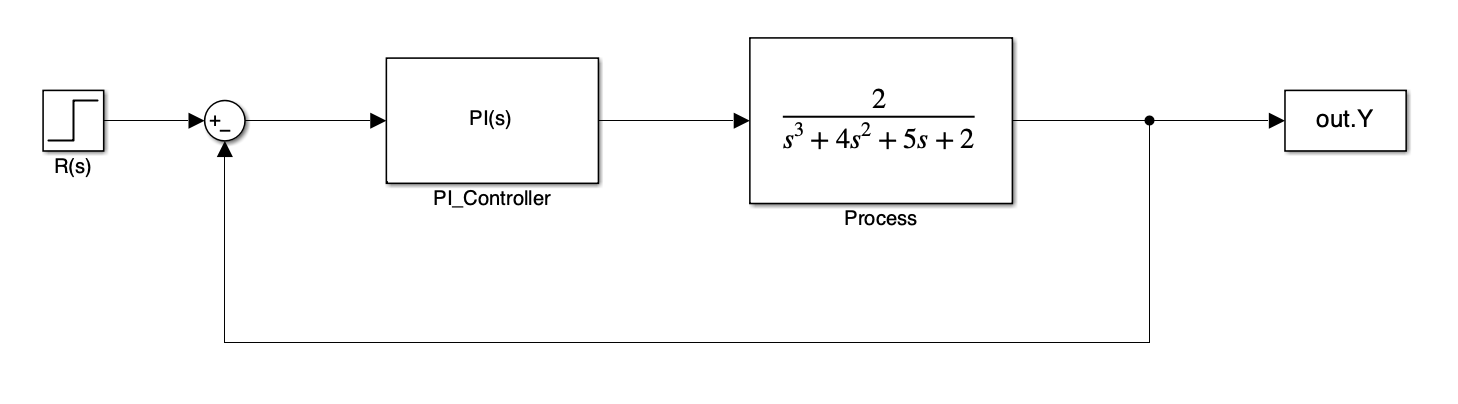
\includegraphics[width=1\textwidth]{Figures/figure1-3a.png}
        \caption{Simulink model of the PI-controlled system.}
      \end{figure}

      \begin{figure}[H]
        \centering
        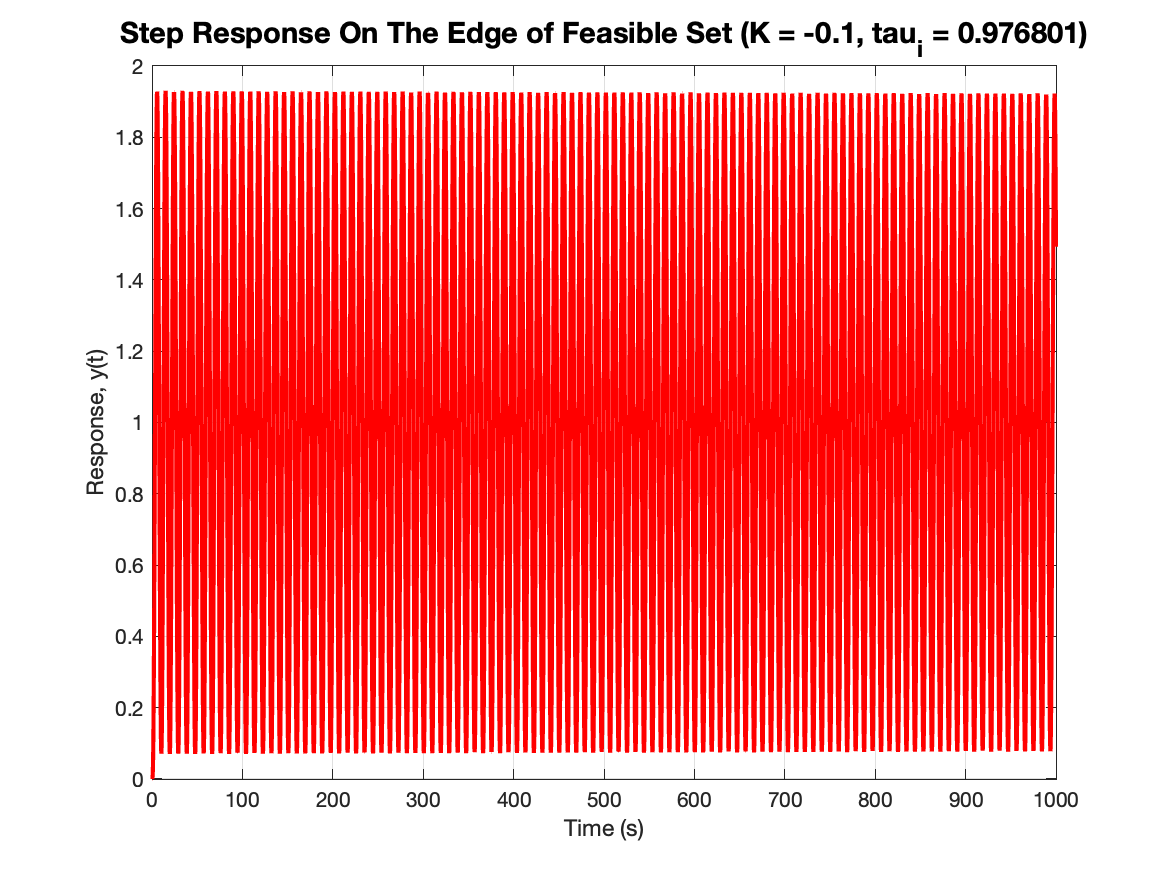
\includegraphics[width=0.7\textwidth]{Figures/figure1-3b.png}
        \caption{Step response on the boundary of the feasible set. The system oscillates and the amplitude grows very slowly, indicating marginal instability.}
      \end{figure}
      
      \begin{figure}[H]
        \centering
        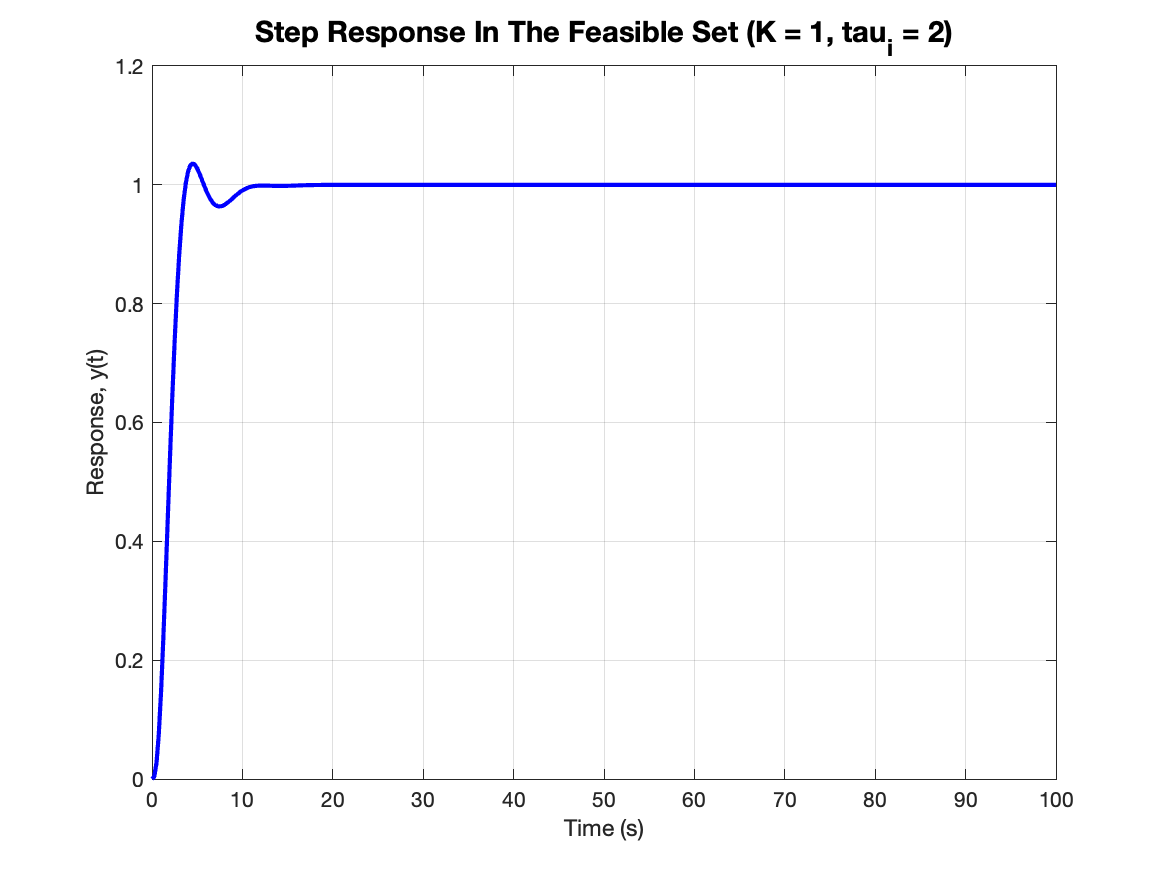
\includegraphics[width=0.7\textwidth]{Figures/figure1-3c.png}
        \caption{Step response for parameters inside the feasible set. The system is stable and relatively well damped, approaching steady state smoothly.}
      \end{figure}
      
      \begin{figure}[H]
        \centering
        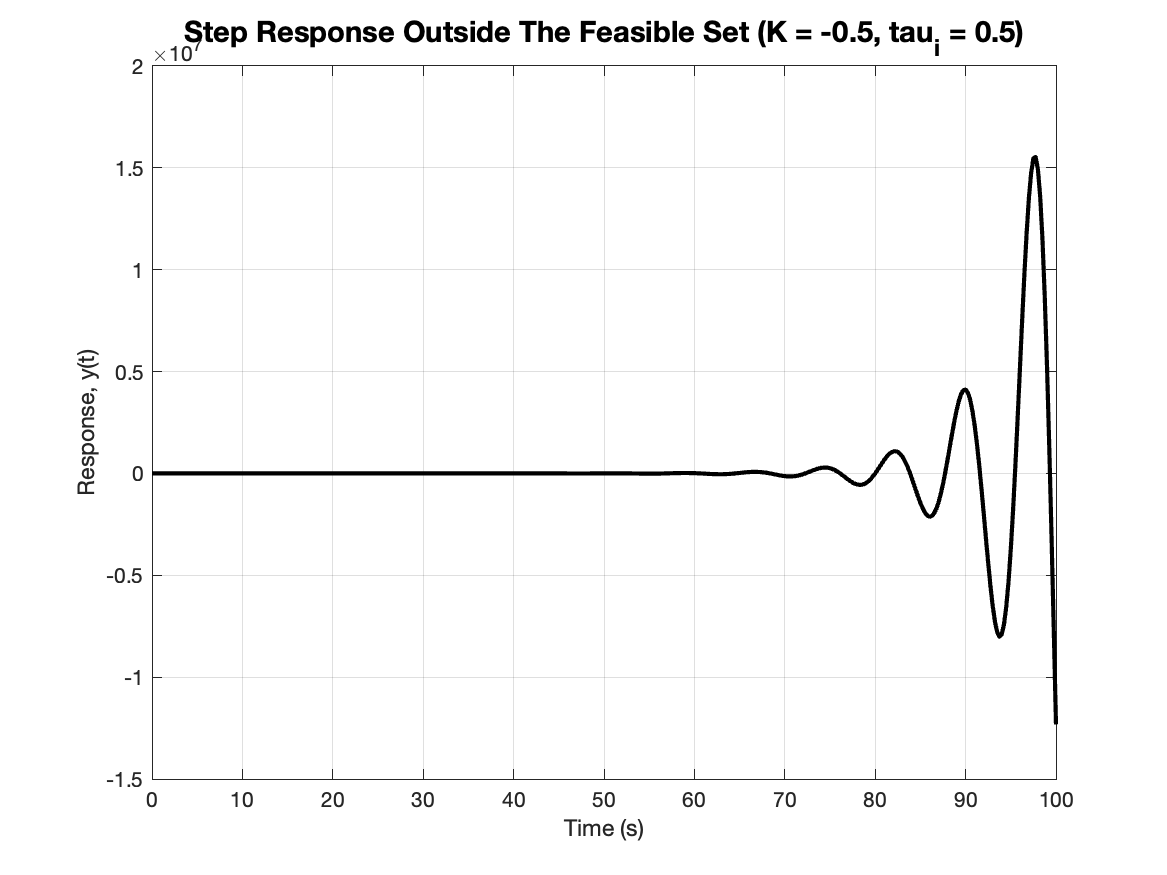
\includegraphics[width=0.7\textwidth]{Figures/figure1-3d.png}
        \caption{Step response for parameters outside the feasible set. The system exhibits fast-growing oscillations, clearly demonstrating instability.}
      \end{figure}
      
      The edge case exhibits slow-growing oscillations, which indicates marginal instability. Although the system initially appears to behave stably, the oscillations increase in amplitude over time. This is consistent with the fact that the chosen parameters lie directly on the boundary of the feasible set, where the Routh-Hurwitz conditions require strict inequalities ($>$) rather than allowing equality. The second case, which is well within the feasible region, produces a stable and mostly well-damped response. The final case, with parameters outside the feasible set, immediately shows rapidly growing oscillations, confirming instability.

      \clearpage
      % Answer to 1.4
      \item 
      The Routh-Hurwitz array was recomputed with the new transport delay (using first-order Padé approximation) to determine how the delay affects system stability.
  
      \begin{figure}[H]
        \centering
        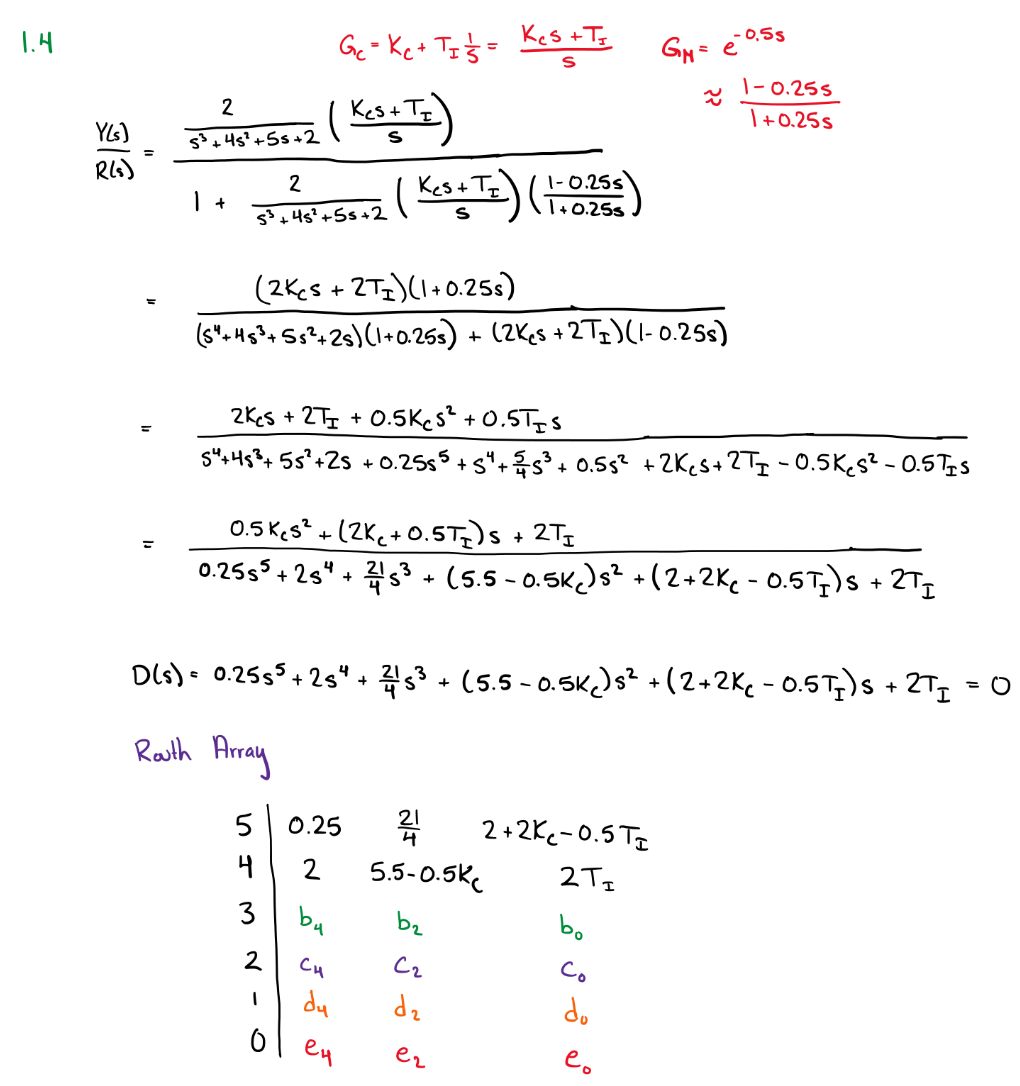
\includegraphics[width=0.9\textwidth]{Figures/figure1-4a.png}
        \caption{Step 1 of Routh Array with transport delay.}
      \end{figure}
  
      \begin{figure}[H]
        \centering
        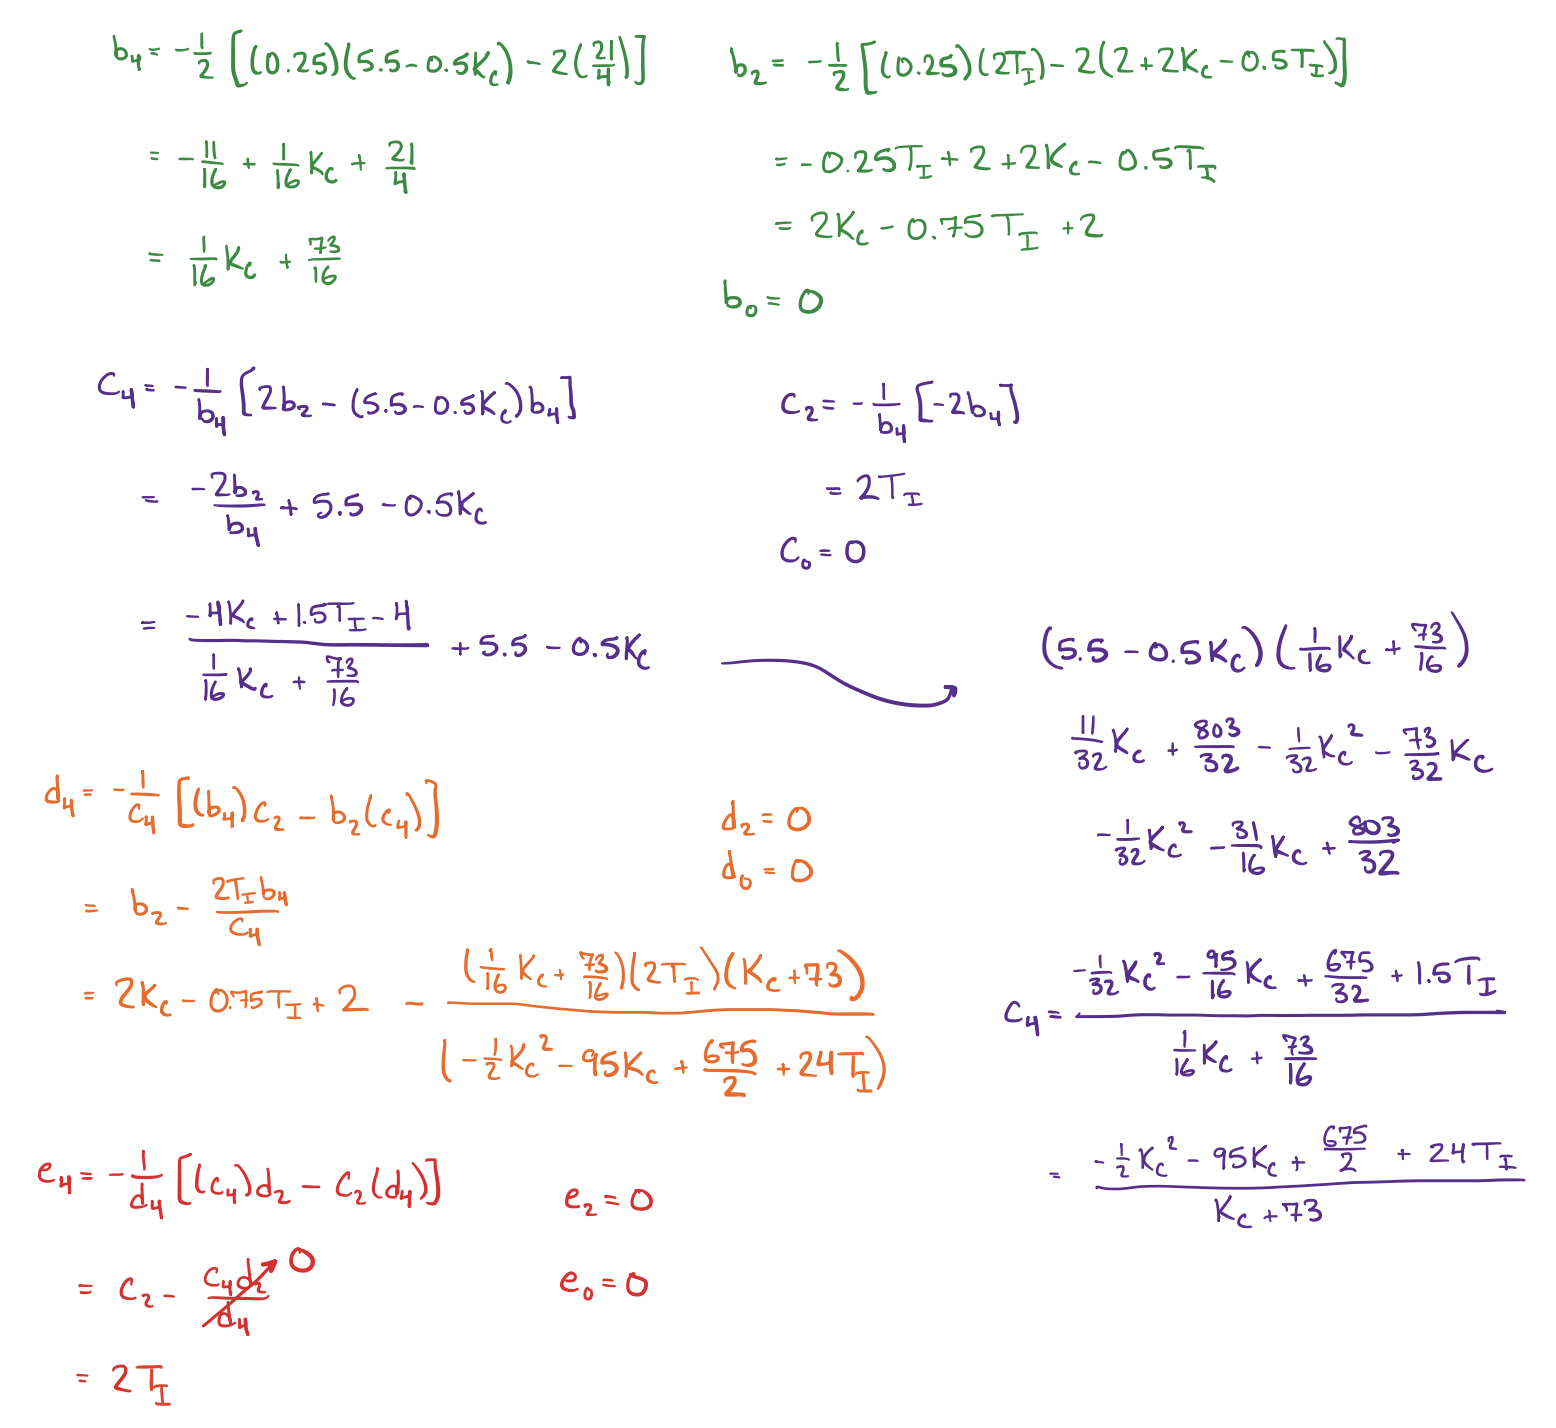
\includegraphics[width=0.9\textwidth]{Figures/figure1-4b.png}
        \caption{Step 2 of Routh Array with transport delay.}
      \end{figure}
  
      \begin{figure}[H]
        \centering
        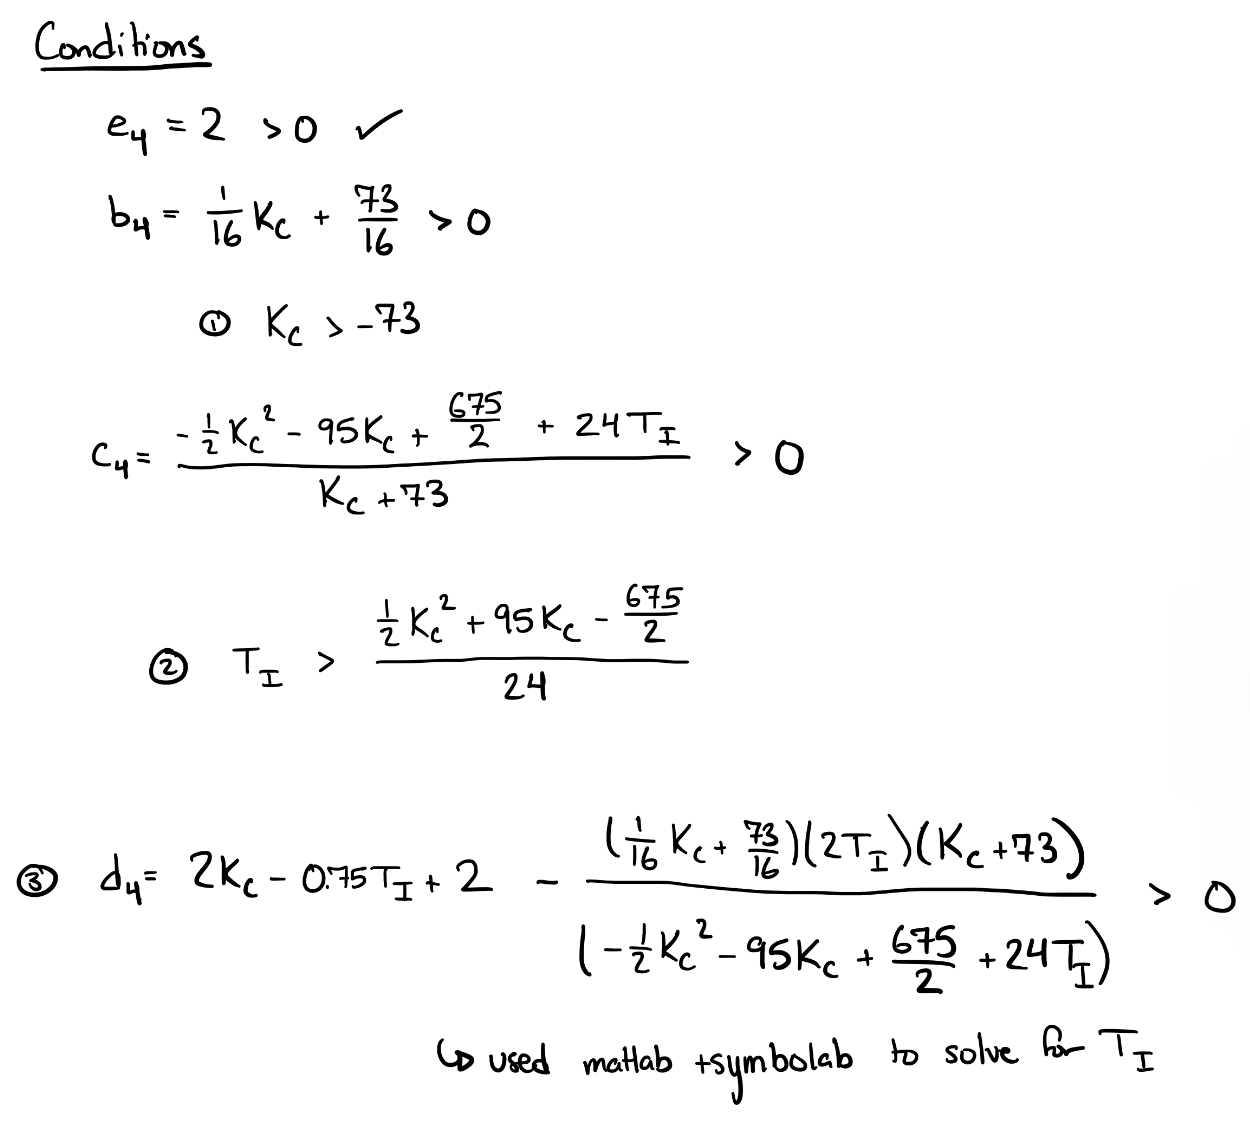
\includegraphics[width=0.8\textwidth]{Figures/figure1-4c.png}
        \caption{Final Routh Array with delay-based conditions.}
      \end{figure}
  
      \begin{figure}[H]
        \centering
        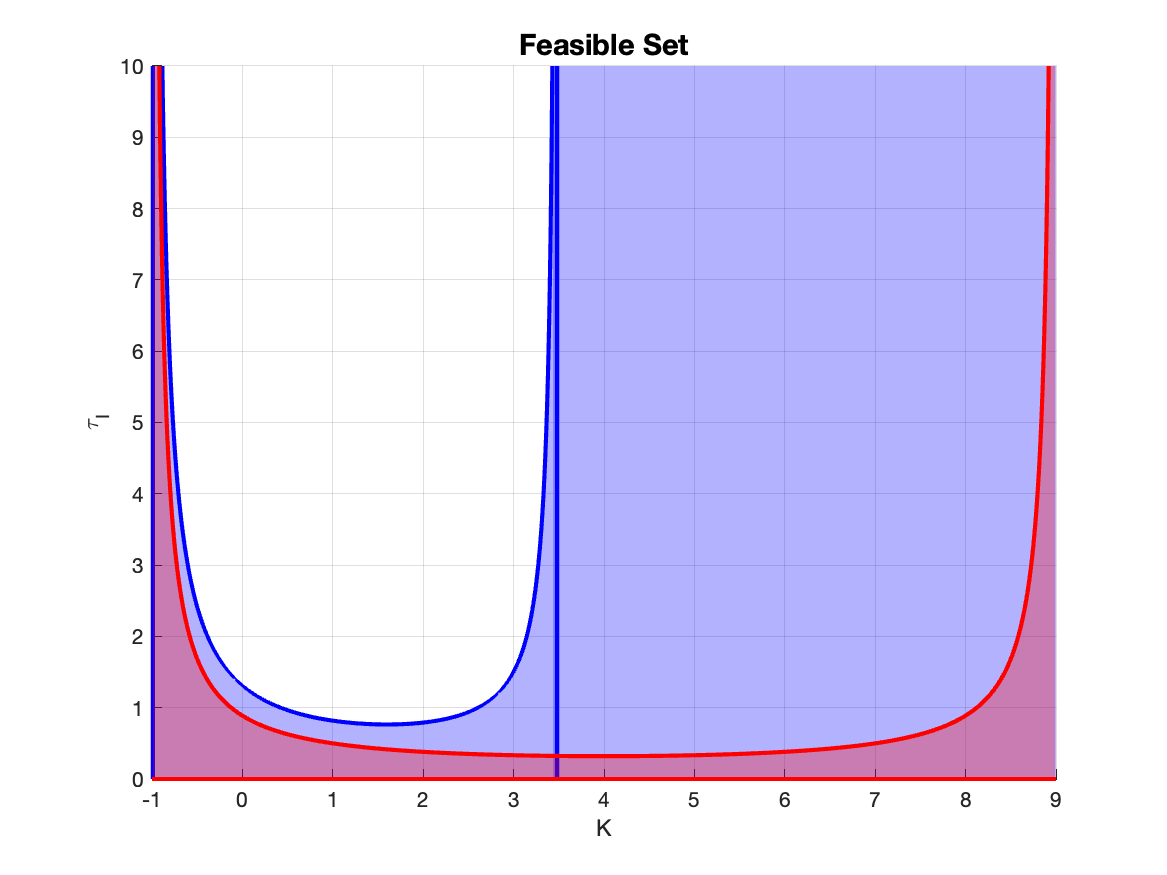
\includegraphics[width=0.8\textwidth]{Figures/figure1-4d.png}
        \caption{Feasible sets with and without delay. Blue indicates infeasible region of the new delayed system. Red is the same infeasible region from earlier.}
      \end{figure}
  
      As seen in the figure, the introduction of transport delay reduces the size of the feasible region, particularly in areas with small integral time $\tau_I$ or large controller gain $K_C$. This is because transport delay introduces additional phase lag into the system, which decreases the phase margin and brings the system closer to instability. From the perspective of the Bode plot, delay shifts the phase curve to the left, meaning that the phase crosses $-180^\circ$ at a lower frequency. This corresponds to a higher critical gain $A_c$, which implies a lower allowable $K_C$ for stability. In practical terms, this means that the system must be detuned ($K_C$ must be reduced) when delay is present. If the gain is not reduced accordingly, the aggressive controller action causes excessive oscillations, and the system approaches instability. This explains why many of the previously stable combinations of $K_C$ and $\tau_I$ now fall outside the feasible set when delay is introduced.

      \clearpage
      % Answer to 1.5
      \item 
      The system was simulated again using the same controller parameters ($K_C=2$, $\tau_I=1$) for both the delay and non-delay versions. These values were chosen by looking at the feasible sets and picking values that lay in both the time delay and non-time delayed feasible sets. The updated Simulink model includes the transport delay block.
  
      \begin{figure}[H]
        \centering
        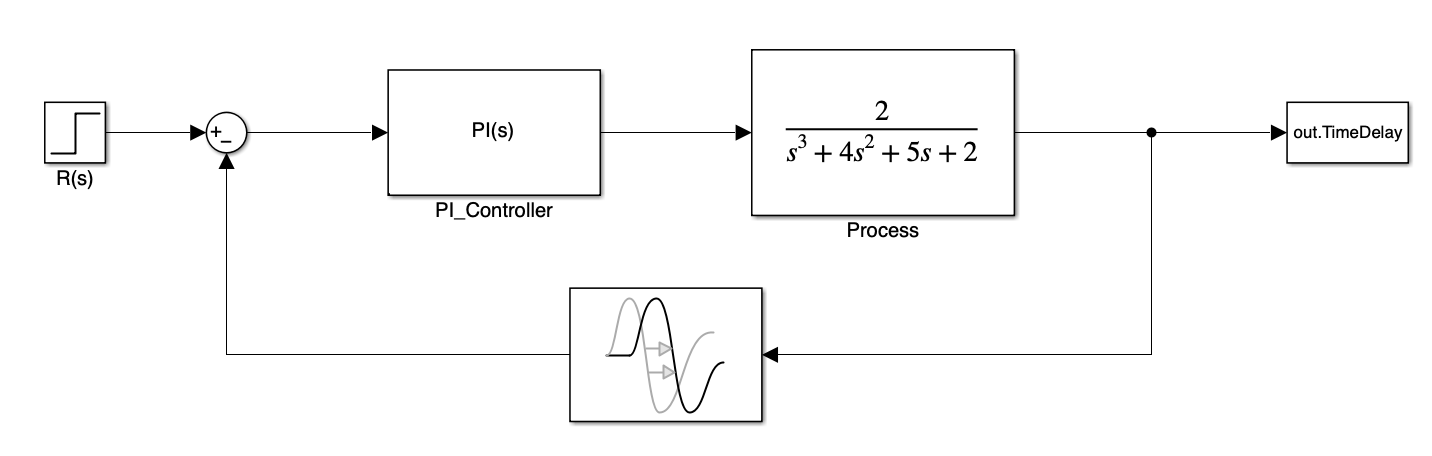
\includegraphics[width=0.9\textwidth]{Figures/figure1-5a.png}
        \caption{Simulink model with transport delay included.}
      \end{figure}
  
      \begin{figure}[H]
        \centering
        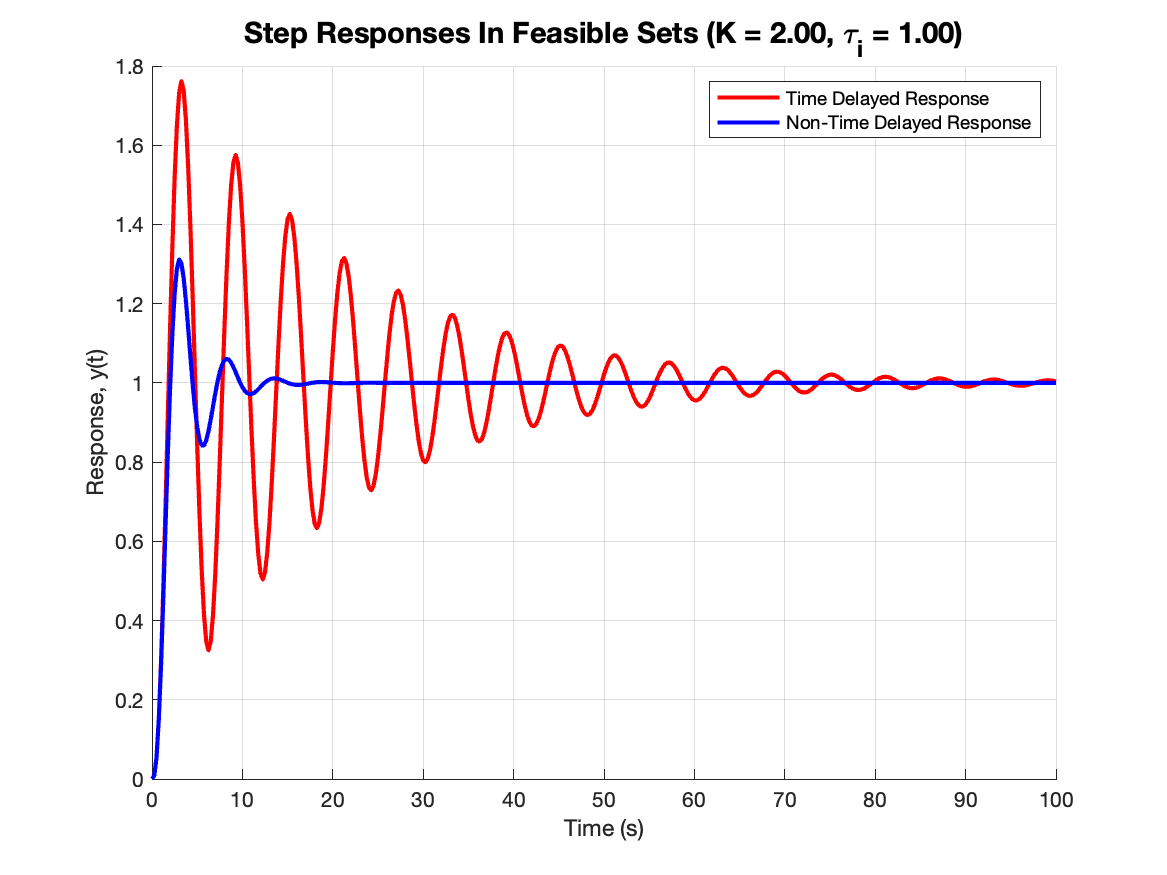
\includegraphics[width=0.8\textwidth]{Figures/figure1-5b.png}
        \caption{Comparison of system response with and without transport delay.}
      \end{figure}
  
      The system with transport delay exhibits more oscillatory behavior and takes longer to settle compared to the delay-free case, despite using identical PI tuning parameters. This aligns with the analysis in 1.4, where the added phase lag from delay was shown to reduce stability margins and narrow the feasible set. The delay effectively pushes the system closer to instability, and without detuning $K_C$, even stable configurations become more oscillatory and sluggish in response.  
    \end{enumerate}
    

\clearpage
\item Question 2
  \begin{enumerate}
    % 2.1
    \item Write answer here
     
  \end{enumerate}

\end{enumerate}

\end{document}
